\documentclass{article}

\usepackage{tikz}
\usepackage{anyfontsize}

\usetikzlibrary{external}
\usetikzlibrary{arrows.meta}
\usetikzlibrary{bending}
\usetikzlibrary{matrix}

\tikzexternalize[verbose=false]
\begin{document}

\tikzsetnextfilename{1-polygon}

\begin{figure}
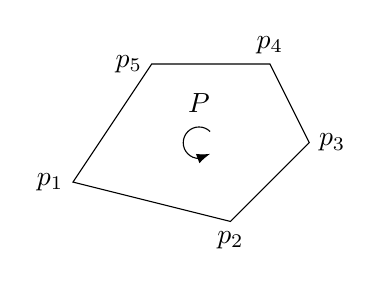
\begin{tikzpicture}
\draw (0,0.5) -- (2, 0) -- (3, 1) -- (2.5, 2) -- (1, 2) -- cycle;
\draw [-Latex] ([shift=(45:0.2)]1.6, 1.0) arc [radius=0.2, start angle=45, end angle= 315];
\node [left] at (1,2) {$p_5$};
\node [left] at (0,0.5) {$p_1$};
\node [below] at (2,0) {$p_2$};
\node [right] at (3,1) {$p_3$};
\node [above] at (2.5,2) {$p_4$};
\node at (1.6, 1.5) {$P$};
\end{tikzpicture}
\end{figure}

\tikzsetnextfilename{1-shoelace}

\begin{figure}
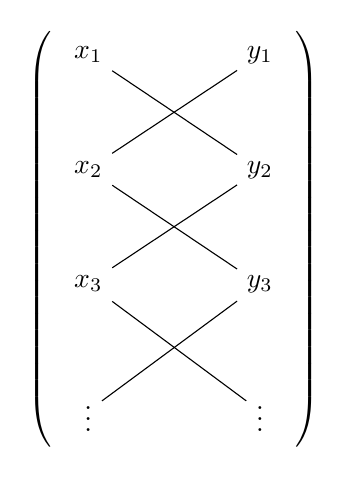
\begin{tikzpicture}
\matrix (M)[matrix of math nodes,row sep=1cm,column sep=16mm,left delimiter=(,right delimiter=)]{
x_1 & y_1 \\ x_2 & y_2 \\ x_3 & y_3 \\ \vdots & \vdots\\
};
\draw (M-1-1)--(M-2-2);
\draw (M-1-2)--(M-2-1);
\draw (M-2-1)--(M-3-2);
\draw (M-2-2)--(M-3-1);
\draw (M-3-1)--(M-4-2);
\draw (M-3-2)--(M-4-1);
\end{tikzpicture}
\end{figure}


\tikzsetnextfilename{2-negative}

\begin{figure}
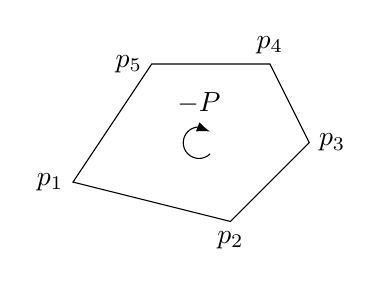
\begin{tikzpicture}
\draw (0,0.5) -- (2, 0) -- (3, 1) -- (2.5, 2) -- (1, 2) -- cycle;
\draw [Latex-] ([shift=(45:0.2)]1.6,1) arc [radius=0.2, start angle=45, end angle= 315];
\node [left] at (1,2) {$p_5$};
\node [left] at (0,0.5) {$p_1$};
\node [below] at (2,0) {$p_2$};
\node [right] at (3,1) {$p_3$};
\node [above] at (2.5,2) {$p_4$};
\node at (1.6, 1.5) {$-P$};
\end{tikzpicture}
\end{figure}


\tikzsetnextfilename{3-subtraction}

\begin{figure}
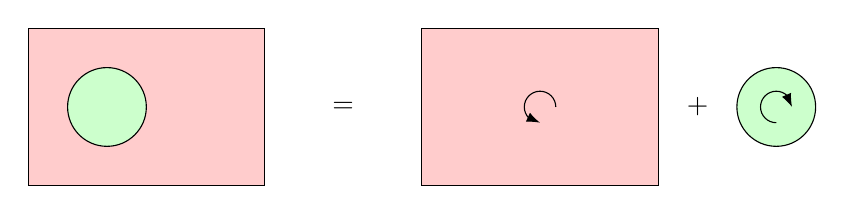
\begin{tikzpicture}
\draw [fill=red!20] (0,0) rectangle ++(3,2);
\draw [fill=green!20] (1,1) circle [radius=0.5];
\node at (4,1) {$=$};
\draw [fill=red!20] (5,0) rectangle ++(3,2);
\draw [-Latex] ([shift=(0:0.2)]6.5,1) arc [radius=0.2, start angle=0, end angle= 270];

\node at (8.5,1) {$+$};
\draw [fill=green!20] (9.5,1) circle [radius=0.5];
\draw [Latex-] ([shift=(0:0.2)]9.5,1) arc [radius=0.2, start angle=0, end angle= 270];
\end{tikzpicture}
\end{figure}

\tikzsetnextfilename{4-triangles}

\begin{figure}
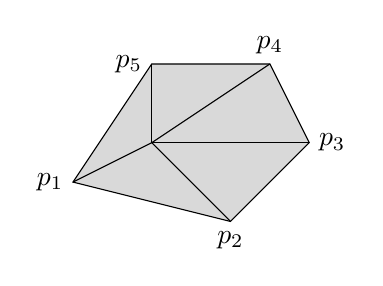
\begin{tikzpicture}
\draw [fill=gray!30] (0,0.5) -- (2, 0) -- (3, 1) -- (2.5, 2) -- (1, 2) -- cycle;
\draw (1,1) -- (0,0.5);
\draw (1,1) -- (2,0);
\draw (1,1) -- (3,1);
\draw (1,1) -- (2.5,2);
\draw (1,1) -- (1,2);
\node [left] at (0,0.5) {$p_1$};
\node [below] at (2,0) {$p_2$};
\node [right] at (3,1) {$p_3$};
\node [above] at (2.5,2) {$p_4$};
\node [left] at (1,2) {$p_5$};
\end{tikzpicture}
\end{figure}

\tikzsetnextfilename{5-triangles2}

\begin{figure}
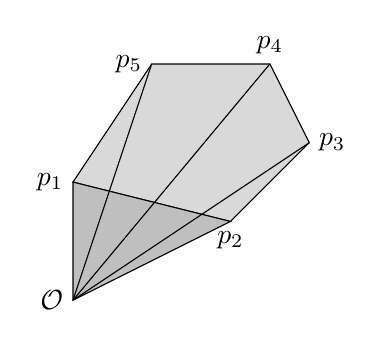
\begin{tikzpicture}
\draw [fill=gray!30] (0,0.5) -- (2, 0) -- (3, 1) -- (2.5, 2) -- (1, 2) -- cycle;
\draw [fill=gray!50] (0,0.5) -- (2,0) -- (0,-1) -- cycle;
\draw (3,1) -- (0,-1);
\draw (2.5,2) -- (0,-1);
\draw (1,2) -- (0,-1);
\node [left] at (0,0.5) {$p_1$};
\node [below] at (2,0) {$p_2$};
\node [right] at (3,1) {$p_3$};
\node [above] at (2.5,2) {$p_4$};
\node [left] at (1,2) {$p_5$};
\node [left] at (0,-1) {$\mathcal{O}$};
\end{tikzpicture}
\end{figure}

\tikzsetnextfilename{6-nonsimple}

\begin{figure}
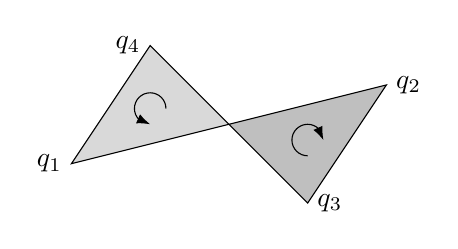
\begin{tikzpicture}
\draw [fill=gray!30] (1, 2) -- (0,0.5) -- (2, 1) -- cycle;
\draw [fill=gray!50] (2,1) -- (4, 1.5) -- (3, 0) -- cycle;
\node [left] at (1,2) {$q_4$};
\node [left] at (0,0.5) {$q_1$};
\node [right] at (4,1.5) {$q_2$};
\node [right] at (3,0) {$q_3$};
\draw [-Latex] ([shift=(0:0.2)]1,1.2) arc [radius=0.2, start angle=0, end angle= 270];
\draw [Latex-] ([shift=(0:0.2)]3,0.8) arc [radius=0.2, start angle=0, end angle= 270];

\end{tikzpicture}
\end{figure}

\tikzsetnextfilename{7-angles}

\begin{figure}
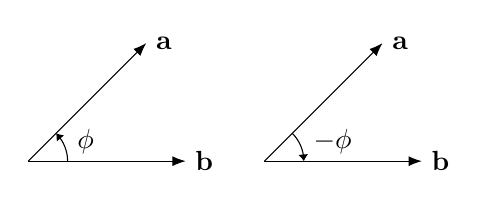
\begin{tikzpicture}
\draw [-Latex] (0,0) -- ++(1.5, 1.5);
\draw [-Latex] (0,0) -- ++(2,0);
\node [right] at (1.5,1.5) {$\bf{a}$};
\node [right] at (2,0) {$\bf{b}$};
\draw [arrows = {-Latex[scale length=0.5]}] ([shift=(0:0.5)]0,0) arc [radius=0.5, start angle=0, end angle= 45];
\node [right] at (0.5, 0.25) {$\phi$};

\draw [-Latex] (3,0) -- ++(1.5, 1.5);
\draw [-Latex] (3,0) -- ++(2, 0);
\node [right] at (4.5,1.5) {$\bf{a}$};
\node [right] at (5, 0) {$\bf{b}$};
\draw [arrows = {-Latex[scale length=0.5]}] ([shift=(45:0.5)]3,0) arc [radius=0.5, start angle=45, end angle= 0];
\node [right] at (3.5, 0.25) {$-\phi$};

\end{tikzpicture}
\end{figure}


\tikzsetnextfilename{8-angle-addition}

\begin{figure}
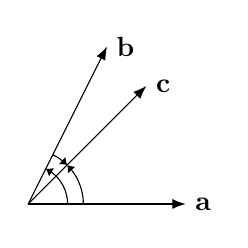
\begin{tikzpicture}
\draw [-Latex] (0,0) -- ++(1.5, 1.5);
\draw [-Latex] (0,0) -- ++(2,0);
\draw [-Latex] (0,0) -- ++(1,2);
\node [right] at (2,0) {$\bf{a}$};
\node [right] at (1,2) {$\bf{b}$};
\node [right] at (1.5,1.5) {$\bf{c}$};
\draw [arrows = {-Latex[scale length=0.5]}] ([shift=(0:0.5)]0,0) arc [radius=0.5, start angle=0, end angle= 63.5];
\draw [arrows = {-Latex[scale length=0.5]}] ([shift=(63.5:0.7)]0,0) arc [radius=0.7, start angle=63.5, end angle= 45];
\draw [arrows = {-Latex[scale length=0.5]}] ([shift=(0:0.7)]0,0) arc [radius=0.7, start angle=0, end angle= 45];

\end{tikzpicture}
\end{figure}



\tikzsetnextfilename{9-displacements}

\begin{figure}
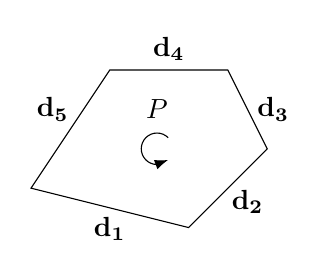
\begin{tikzpicture}
\draw (0,0.5) -- (2, 0) -- (3, 1) -- (2.5, 2) -- (1, 2) -- cycle;
\draw [-Latex] ([shift=(45:0.2)]1.6, 1.0) arc [radius=0.2, start angle=45, end angle= 315];
\node [left] at (0.6,1.5) {$\bf{d}_5$};
\node [below] at (1,0.25) {$\bf{d}_1$};
\node [below] at (2.75,0.6) {$\bf{d}_2$};
\node [right] at (2.75,1.5) {$\bf{d}_3$};
\node [above] at (1.75,2) {$\bf{d}_4$};
\node at (1.6, 1.5) {$P$};
\end{tikzpicture}
\end{figure}

\tikzsetnextfilename{9-displacements2}

\begin{figure}
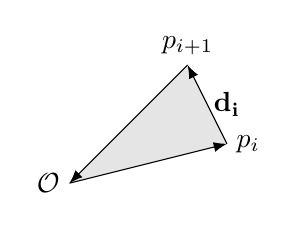
\begin{tikzpicture}

\path [fill=gray!20] (0,0) -- (2,0.5) -- (1.5,1.5) -- cycle;
\draw [-Latex] (0,0) -- (2,0.5);
\node [right] at (2,0.5) {$p_i$};
\draw [Latex-] (0,0) -- (1.5,1.5);
\node [above] at (1.5,1.5) {$p_{i+1}$};
\draw [-Latex] (2, 0.5) -- (1.5,1.5);
\node at (2, 1) {$\bf{d}_i$};
\node [left] at (0,0) {$\mathcal{O}$};

\end{tikzpicture}
\end{figure}


\tikzsetnextfilename{10-interior}

\begin{figure}
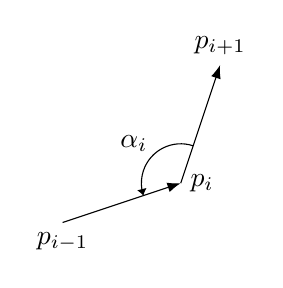
\begin{tikzpicture}

\node [below] at (0,0) {$p_{i-1}$};
\draw [-Latex] (0,0) -- (1.5,0.5);
\node [right] at (1.5,0.5) {$p_i$};
\draw [-Latex] (1.5,0.5) -- (2,2);
\node [above] at (2, 2) {$p_{i+1}$};
\draw [arrows = {-Latex[scale length=0.5]}] ([shift=(71.5:0.5)]1.5,0.5) arc [radius=0.5, start angle=71.5, end angle= 198.5];
\node [left] at (1.2, 1) {$\alpha_i$};


\end{tikzpicture}
\end{figure}

\tikzsetnextfilename{11-regular}

\begin{figure}
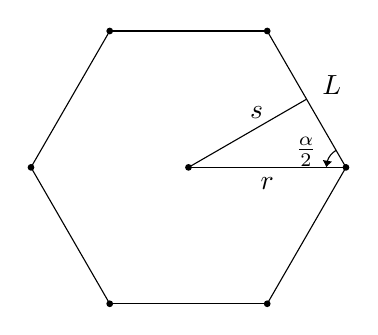
\begin{tikzpicture}

\foreach \a in {0,60,...,300} { 
	\draw[fill] (\a:2) circle (1pt);
	\draw (\a:2) -- (\a+60: 2);
}
\draw[fill] (0,0) circle(1pt);
\draw [arrows = {-Latex[scale length=0.5]}] ([shift=(120:0.25)]2,0) arc [radius=0.25, start angle=120, end angle= 180];
\node[left] at (1.75,0.2) {$\frac{\alpha}{2}$};
\draw (0,0) -- ([shift=(120:1)]2,0);
\draw (0,0) -- (2,0);

\node (above) at ([shift=(30:1)]0,0.2) {$s$};
\node (below) at (1,-0.2) {$r$};
\node (above) at ([shift=(30:2.1)]0,0) {$L$};

\end{tikzpicture}
\end{figure}

\tikzsetnextfilename{11-exterior}

\begin{figure}
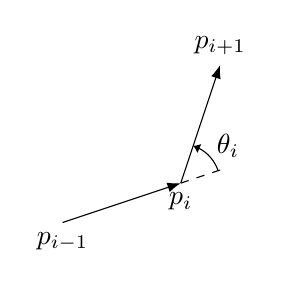
\begin{tikzpicture}

\node [below] at (0,0) {$p_{i-1}$};
\draw [-Latex] (0,0) -- (1.5,0.5);
\node [below] at (1.5,0.5) {$p_i$};
\draw [-Latex] (1.5,0.5) -- (2,2);
\node [above] at (2, 2) {$p_{i+1}$};

\draw[dashed] (1.5,0.5) -- (2.1, 0.7);
\draw [arrows = {-Latex[scale length=0.5]}] ([shift=(18.5:0.5)]1.5,0.5) arc [radius=0.5, start angle=18.5, end angle= 71.5];
\node [above] at (2.1, 0.7) {$\theta_i$};

\end{tikzpicture}
\end{figure}

\tikzsetnextfilename{12-exterior2}

\begin{figure}
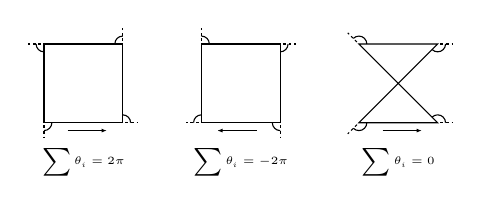
\begin{tikzpicture}[dash1/.style={dashed,dash pattern=on 1pt off 1pt, dash phase=1pt}, font=\fontsize{4}{4}\selectfont]

\draw (0,0) -- (1,0) -- (1,1) -- (0,1) -- cycle;
\draw[dash1] (0,0) -- (0,-0.2);
\draw[dash1] (1,0) -- (1.2,0);
\draw[dash1] (1,1) -- (1,1.2);
\draw[dash1] (0,1) -- (-0.2,1);

\draw ([shift=(270:0.1)]0,0) arc [radius=0.1, start angle=-90, end angle= 0  ];
\draw ([shift=(0  :0.1)]1,0) arc [radius=0.1, start angle=0  , end angle= 90 ];
\draw ([shift=(90 :0.1)]1,1) arc [radius=0.1, start angle=90 , end angle= 180];
\draw ([shift=(180:0.1)]0,1) arc [radius=0.1, start angle=180, end angle= 270];

\draw [arrows = {-Latex[scale=0.4]}] (0.3, -0.1) -- (0.8, -0.1);
\node at (0.5,-0.5) {$\sum \theta_i = 2\pi$};

\draw (2,0) -- (3,0) -- (3,1) -- (2,1) -- cycle;
\draw[dash1] (2,0) -- (1.8,0);
\draw[dash1] (3,0) -- (3,-0.2);
\draw[dash1] (3,1) -- (3.2,1);
\draw[dash1] (2,1) -- (2,1.2);

\draw [arrows = {-Latex[scale=0.4]}] (2.7, -0.1) -- (2.2, -0.1);
\node at (2.5,-0.5) {$\sum \theta_i = -2\pi$};

\draw ([shift=(180:0.1)]2,0) arc [radius=0.1, start angle=180, end angle= 90 ];
\draw ([shift=(90 :0.1)]2,1) arc [radius=0.1, start angle=90 , end angle= 0 ];
\draw ([shift=(0 :0.1)]3,1) arc [radius=0.1, start angle=0 , end angle= -90];
\draw ([shift=(-90:0.1)]3,0) arc [radius=0.1, start angle=-90, end angle=-180];

\draw [arrows = {-Latex[scale=0.4]}] (4.3, -0.1) -- (4.8, -0.1);
\node at (4.5,-0.5) {$\sum \theta_i = 0$};

\draw (4,0) -- (5,0) -- (4,1) -- (5,1) -- cycle;
\draw[dash1] (4,0) -- ([shift=(225:0.2)]4,0);
\draw[dash1] (5,0) -- (5.2,0);
\draw[dash1] (4,1) -- ([shift=(135:0.2)]4,1);
\draw[dash1] (5,1) -- (5.2,1);

\draw ([shift=(-135:0.1)]4,0) arc [radius=0.1, start angle=-135, end angle= 0 ];
\draw ([shift=(0 :0.1)]5,0) arc [radius=0.1, start angle=0 , end angle= 135 ];
\draw ([shift=(135  :0.1)]4,1) arc [radius=0.1, start angle=135 , end angle= 0];
\draw ([shift=(0:0.1)]5,1) arc [radius=0.1, start angle=0, end angle= -135];

\end{tikzpicture}
\end{figure}

\tikzsetnextfilename{13-slope}

\begin{figure}
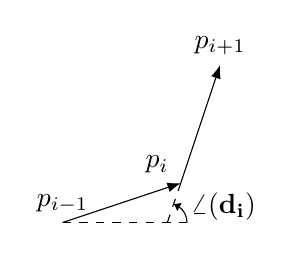
\begin{tikzpicture}

\draw [dashed] (0,0) -- (1.6, 0);
\node [above] at (0,0) {$p_{i-1}$};
\draw [-Latex] (0,0) -- (1.5,0.5);
\node [above] at (1.2,0.5) {$p_i$};
\draw [-Latex] (1.5,0.5) -- (2,2);
\node [above] at (2, 2) {$p_{i+1}$};


\draw[dashed] (1.33,0) -- (1.5, 0.5);
\draw [arrows = {-Latex[scale length=0.5]}] ([shift=(0:0.25)]1.33,0) arc [radius=0.25, start angle=0, end angle= 71.5];
\node [right] at (1.5, 0.2) {$\angle (\bf{d}_i)$};

\end{tikzpicture}
\end{figure}

\tikzsetnextfilename{14-triangle}

\begin{figure}
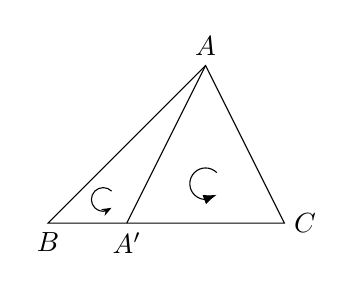
\begin{tikzpicture}

\draw (0,0) -- (3,0) -- (2,2) -- cycle;
\draw (1,0) -- (2,2);
\node [below] at (0,0) {$B$};
\node [above] at (2,2) {$A$};
\node [below] at (1,0) {$A'$};
\node [right] at (3,0) {$C$};

\draw [-Latex] ([shift=(45:0.2)]2,0.5) arc [radius=0.2, start angle=45, end angle= 315];
\draw [arrows = {-Stealth[scale=0.75]}] ([shift=(45:0.15)]0.7,0.3) arc [radius=0.15, start angle=45, end angle= 315];

\end{tikzpicture}
\end{figure}

\tikzsetnextfilename{15-triangle2}

\begin{figure}
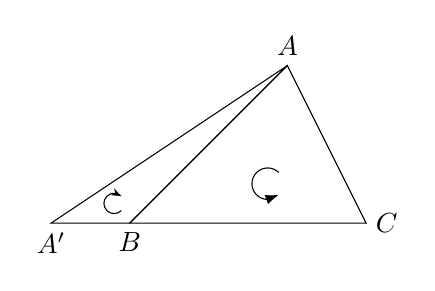
\begin{tikzpicture}

\draw (0,0) -- (3,0) -- (2,2) -- cycle;
\draw (-1,0) -- (0,0) -- (2,2) -- cycle;
\node [below] at (0,0) {$B$};
\node [above] at (2,2) {$A$};
\node [below] at (-1,0) {$A'$};
\node [right] at (3,0) {$C$};

\draw [-Latex] ([shift=(45:0.2)]1.75,0.5) arc [radius=0.2, start angle=45, end angle= 315];
\draw [arrows = {-Stealth[scale=0.75]}]  ([shift=(315:0.13)]-0.2,0.25) arc [radius=0.13, start angle=315, end angle= 45];


\end{tikzpicture}
\end{figure}

\end{document}
